\chapter[Short Chap title]{Empirical study and results}
\section{Data}
This paper considers 1,418 stocks of listing US companies that traded consecutively in the NYSE and NASDAQ stock market of US from January 4, 2016 to December 30, 2016 and uses daily closing price during this period.
% 写一下EIO数据的来源和时间

\section{Network construction}
This paper first calculated normalised direct requirement and normalised direct demand values for every sectors using formula~\ref{equ:eio_i} and formula~\ref{equ:eio_o} and cross-correlation coefficients between every stock pairs using formula~\ref{equ:corr}.

According to the figure~\ref{fig:eio_transaction_density}, the transaction densities decrease as threshold of normalised direct requirement and normalised direct demand increase, and their patterns are exactly similar with the same inflection point at around $threshold=0.136$ where the densities begin to decline. Therefore, the values of thresholds for normalised direct requirement and normalised direct demand are set to be same, i.e., $\theta_{DD}=\theta_{DR}=\theta_{EIO}$,  to filter the directed edges among the stock network.

\begin{figure}
	\begin{center}
		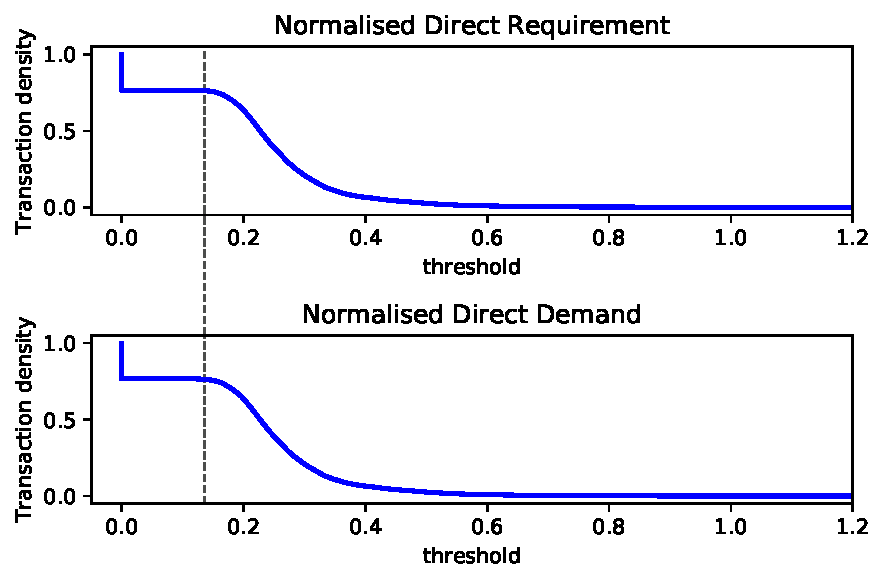
\includegraphics[width=14cm]{eio_transaction_density}
	\end{center}
	\caption{Transaction densities}
	\label{fig:eio_transaction_density}
\end{figure}

\begin{figure}
	\begin{center}
		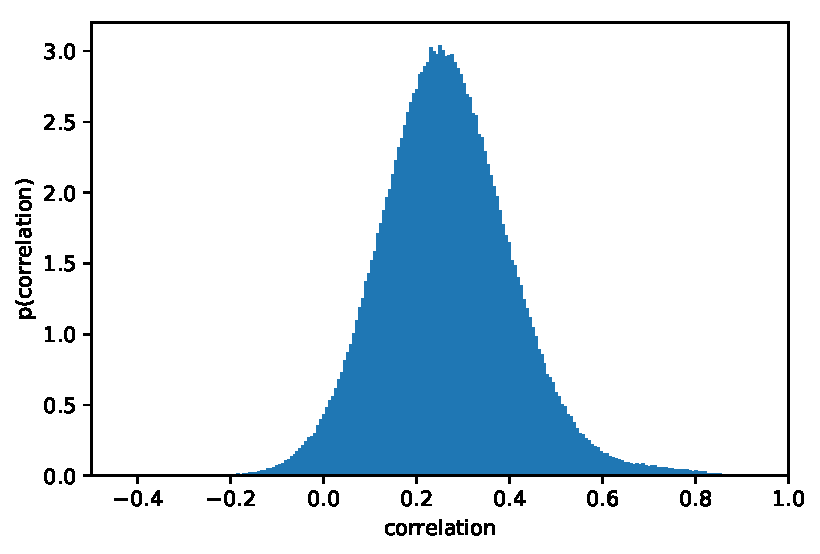
\includegraphics[width=14cm]{correlation_distribution}
	\end{center}
	\caption{Stock price return correlation coefficient distribution}
	\label{fig:correlation_distribution}  
\end{figure}

\begin{figure}
	\begin{center}
		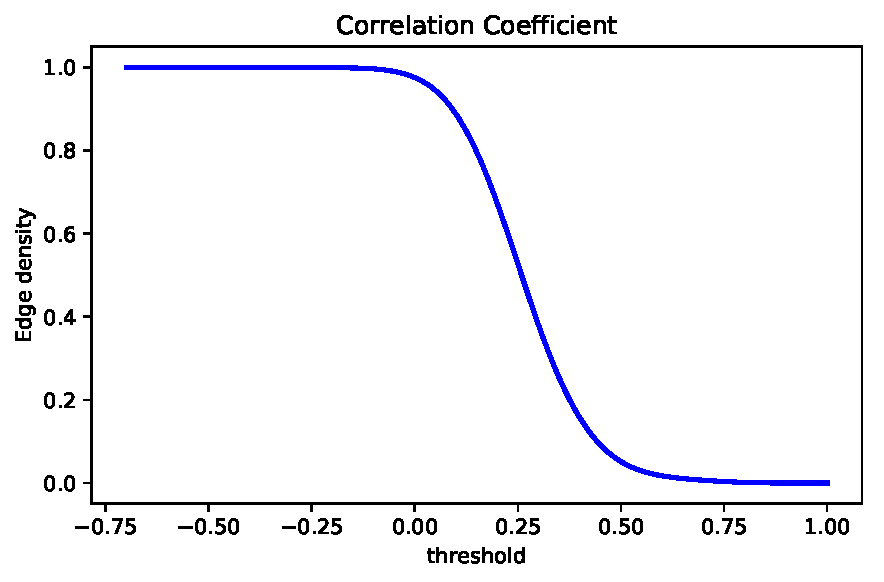
\includegraphics[width=14cm]{correlation_edge_density}
	\end{center}
	\caption{}
	\label{fig:correlation_edge_density}  
\end{figure}

Figure~\ref{fig:correlation_distribution} shows the distribution of stock price correlation coefficients has a shape complies to the normal distribution for the long tails. The correlation coefficients are vary from -0.687 to 0.977 with the mean of 0.265. It implies that the prices of most stocks traded in NYSE and NASDAQ usually fluctuate to the same direction.

% 拟合正态分布或t分布

\begin{figure}
	\begin{center}
		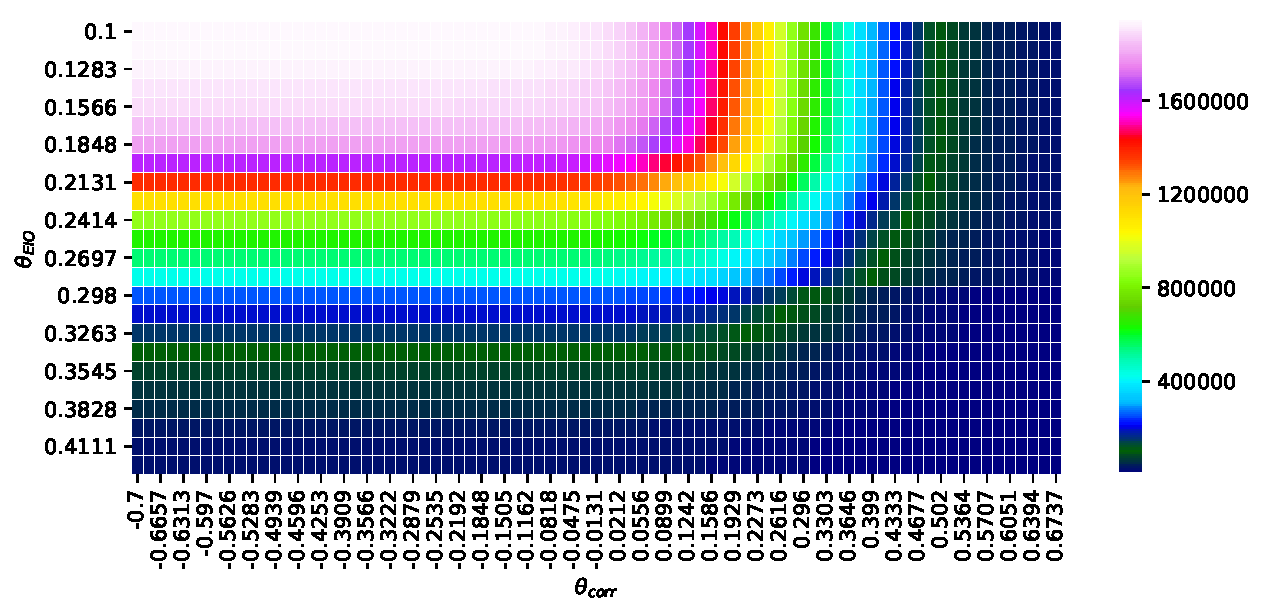
\includegraphics[width=15cm]{amounts_of_edges_threshold}
	\end{center}
	\caption{Numbers of directed edges per EIO-threshold and correlation-coefficient-threshold}
	\label{fig:amounts_of_edges_threshold}  
\end{figure}

Figure~\ref{fig:amounts_of_edges_threshold} shows the number of directed edges remain in the conditions of different value combinations of $\theta_{EIO}$ and $\theta_{corr}$. When both of the thresholds set to be minimal at their own value range, i.e., $\theta_{EIO}=0$ and $\theta_{corr}=-1$, the number of directed edges is $N\times(N-1)=2,009,306$, while $N$ indicates the total number of nodes. According to the figure~\ref{fig:amounts_of_edges_threshold}, the number of edges will be less than 100,000, in which case the network has a density of less than 5\%, if $\theta_{EIO}$ is larger than 0.3545 or $\theta_{corr}$ is larger than 0.5020. 

\begin{figure}
	\begin{center}
		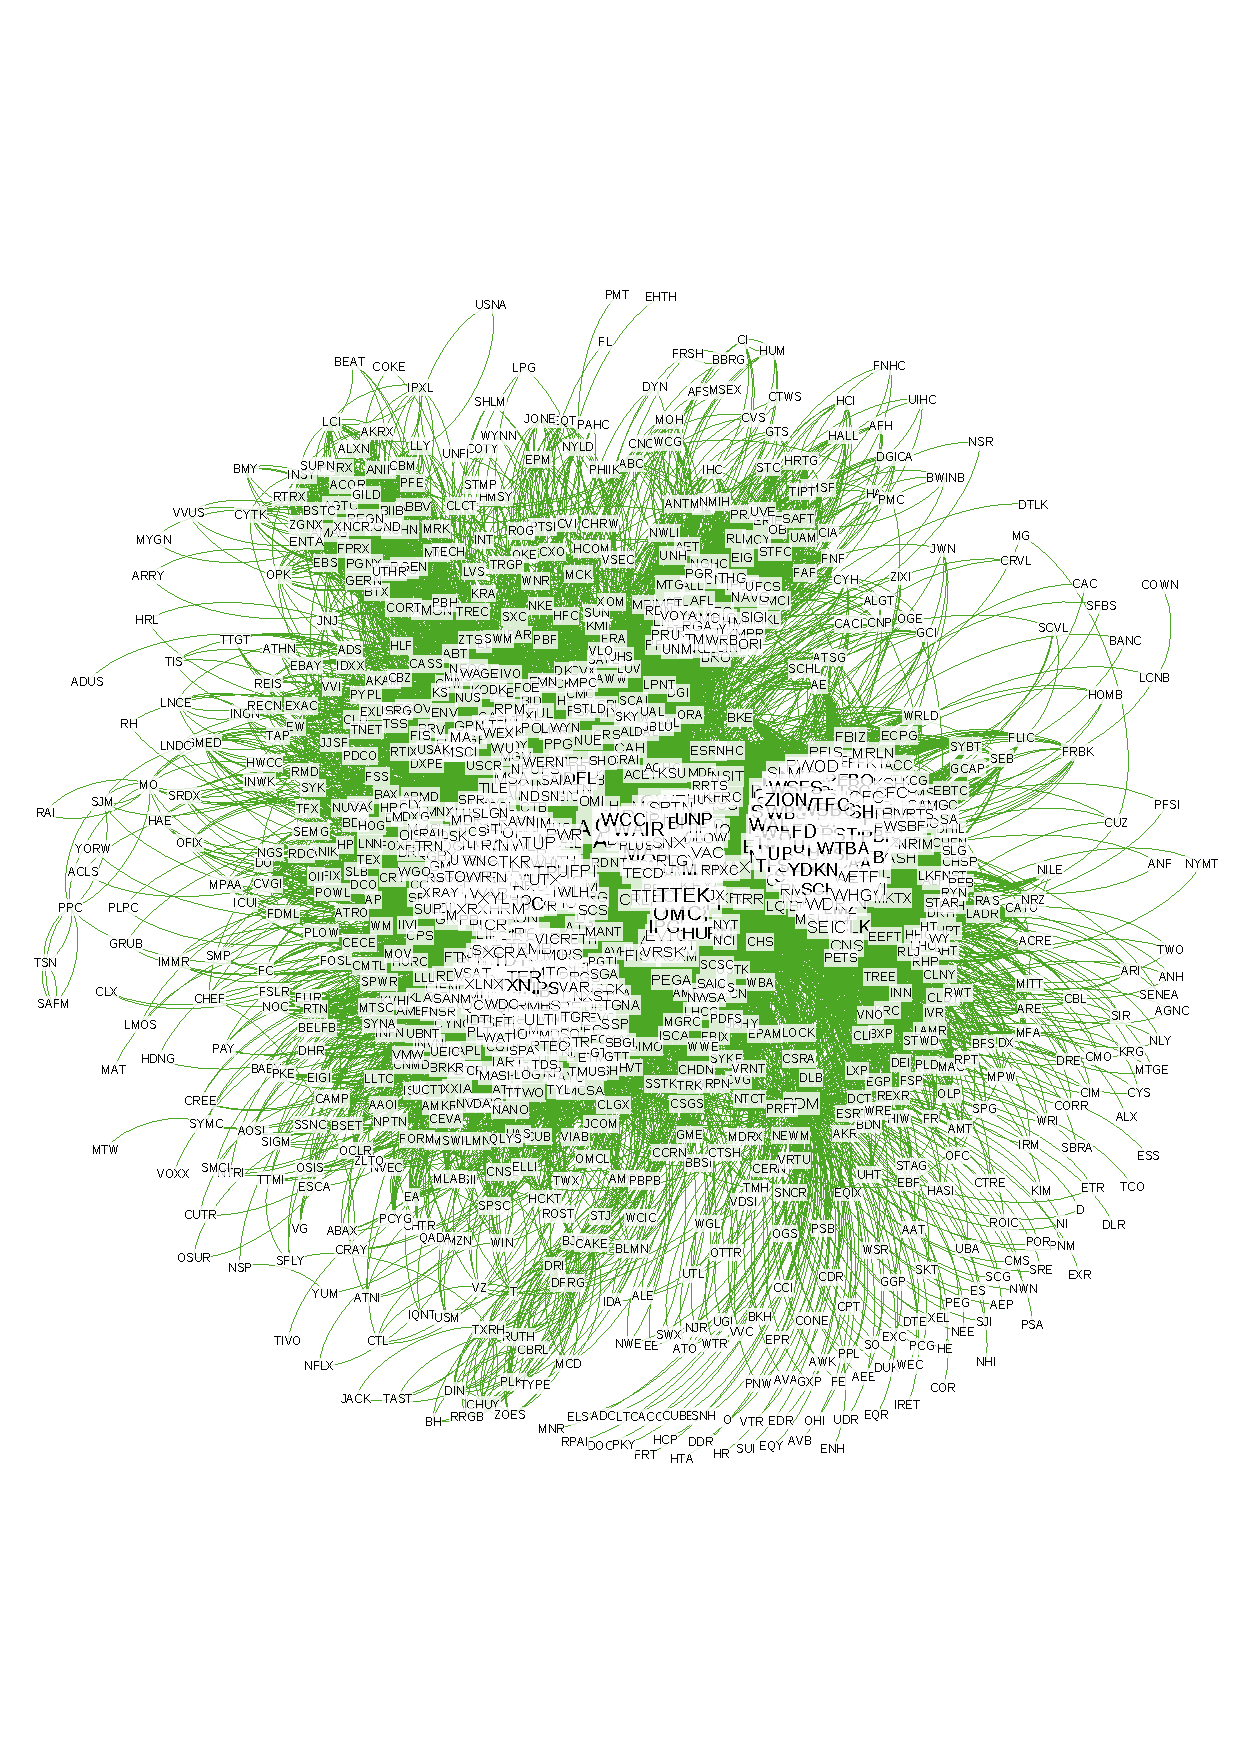
\includegraphics[width=14cm]{Graph_01}
	\end{center}
	\caption{Transaction densities}
	\label{fig:Graph_01}
\end{figure}


It is obvious that the larger values assigned to $\theta_{EIO}$ and $\theta_{corr}$, the more significant for the weights and directions of the remaining edges. But if the network is too sparse, it can not be strongly or weakly connected hence the network becomes inefficient. As a result, this paper selects the threshold-value-pair $\theta_{EIO}=0.292$ and $\theta_{corr}=0.379$ to construct directed unweighted stock network and directed weighted stock network.

%这里放Gephi的图片 可以随机选择一半的结点作为生成

\section{Analysis of the directed unweighted network}
% 对幂指数分布的统计检验
A directed Watts Strogatz small-world network and a random network with the same number of nodes and edges with the stock directed unweighted network are generated. Table~\ref{tab:three} compares the main topologies of the three different networks.

\begin{table}
	\begin{center}
		\begin{tabular}{|r|c|c|c|}\hline\hline
			Directed networks&Stock network&Small-world network&Random network\\\hline
			Number of nodes&1418&1418&1418\\
			Number of edges&102051&102088&102097\\
			Out-degree distribution&Power-law&Normal&Normal\\
			Average out-degrees&143.94&143.99&144.00\\
			Average path length&2.775&2.005&1.973\\
			Clustering coefficient&0.4675&0.1367&0.05105\\
			Global efficiency&0.2563&0.5161&0.5216\\
			Local efficiency&0.6276&0.5027&0.4456\\
			Assortativity&0.02004&-0.002180&0.001452\\
			\hline\hline
		\end{tabular}
	\end{center}
	\caption{Main properties of stock network, small-world network, and random network}\label{tab:three}
\end{table}

\subsection{Power-law distribution}
According to the table~\ref{tab:three}, the values of average out-degrees of stock network, small-world network and random network are almost the same due to the similar number of nodes and edges, but in terms of the distributions of out-degrees, stock network is different from the others. 

Figure~\ref{fig:distributionsm} and \ref{fig:distributionrd} show clearly that the out-degree distribution of small-world network and random network follow the normal distribution, i.e, most degree numbers of nodes fall in the middle range, while figure~\ref{fig:G_out_degree_distribution_square} illustrates that for the stock network, only a few number of nodes show higher out-degree, while most nodes are in the positions of low out-degree level. The distribution of the directed stock price return networks follows power-law distribution with the exponent of 4.057.

%Power-law distribution reveals that most of the nodes have a small degree while a few modes have a higher degree.
\subsection{Small-world property}
The average path length of small-world network and random network are both close to 2, indicates that taking any node in the network, it can expect to reach any other nodes just through one node as medium. For stock network, the expectation number of medium nodes is 1.775, which is also a small number for connection, so like small-world and random networks, stock network also has the small-world property.

% Efficiency.
\subsection{Community feature}
The larger value of clustering coefficient for stock network than the other two networks indicating that the nodes in stock network tend to cluster together. Therefore, communities of stock network will be identified implementing the community detection algorithm for directed networks in this section. According to the industrial sectors to which most component stocks are belong, as figure~\ref{fig:community_sector_stacked} shows, following five communities are identified: (1) Production (2) Finance (3) Livelihood (4) Insurance and chemical products (5) Utilities and financial vehicles.

It can see from figure~\ref{fig:community_graph} that the community of finance (green) has a very dense structure, connected closely inside and completely exclusive from other communities. The communities of production (purple) and livelihood (blue) are sparsely distributed while there are some large-sized nodes acting as hubs of the overall network. The other two communities are more interesting because they have peculiar structures.

Every industrial sectors of individual stocks in community are identified to investigate the properties of the community of insurance and chemical products (yellow). As figure~\ref{fig:community_4} illustrates and through the investigation, most firms in the upper and lower clusters are in the sectors of "chemical products" and "Insurance carriers and related activities" respectively, while firms between the two big clusters, like "MCK" (McKesson) and "CAH" (Cardinal Health), are large medical supplier, pharmaceutical and heathcare service companies with high out-degrees to both of the two clusters. Apart from that, there are also considerable number of links from the upper cluster to the hubs of chemical companies. Thus, it is reasonable to infer that the prices of medicines have significant influence to medical insurance industry, additionally the purchases of chemical products of pharmaceutical firms and the sales of chemical products have made pharmaceutical and chemical companies influence to each other.

Another investigation towards the community of utilities and financial vehicles (orange) is conducted by the same measure. As figure~\ref{fig:community_5} illustrates, there is one huge hub (PDM) which is the company "Piedmont Office Realty Trust" among the community while all the others are one-degree nodes located remotely. More links from the hub to the rest than the opposite direction, and also the weights of the former links are generally higher. The hub, "Piedmont Office Realty Trust", is a real estate investment trust company, and the rest in the community contains 59 "Funds, trusts, and other financial vehicles" firms and 44 "Utilities" firms. % infer

Although the assortativity values for the three networks are all non-significant, 

\begin{figure}
	\begin{center}
		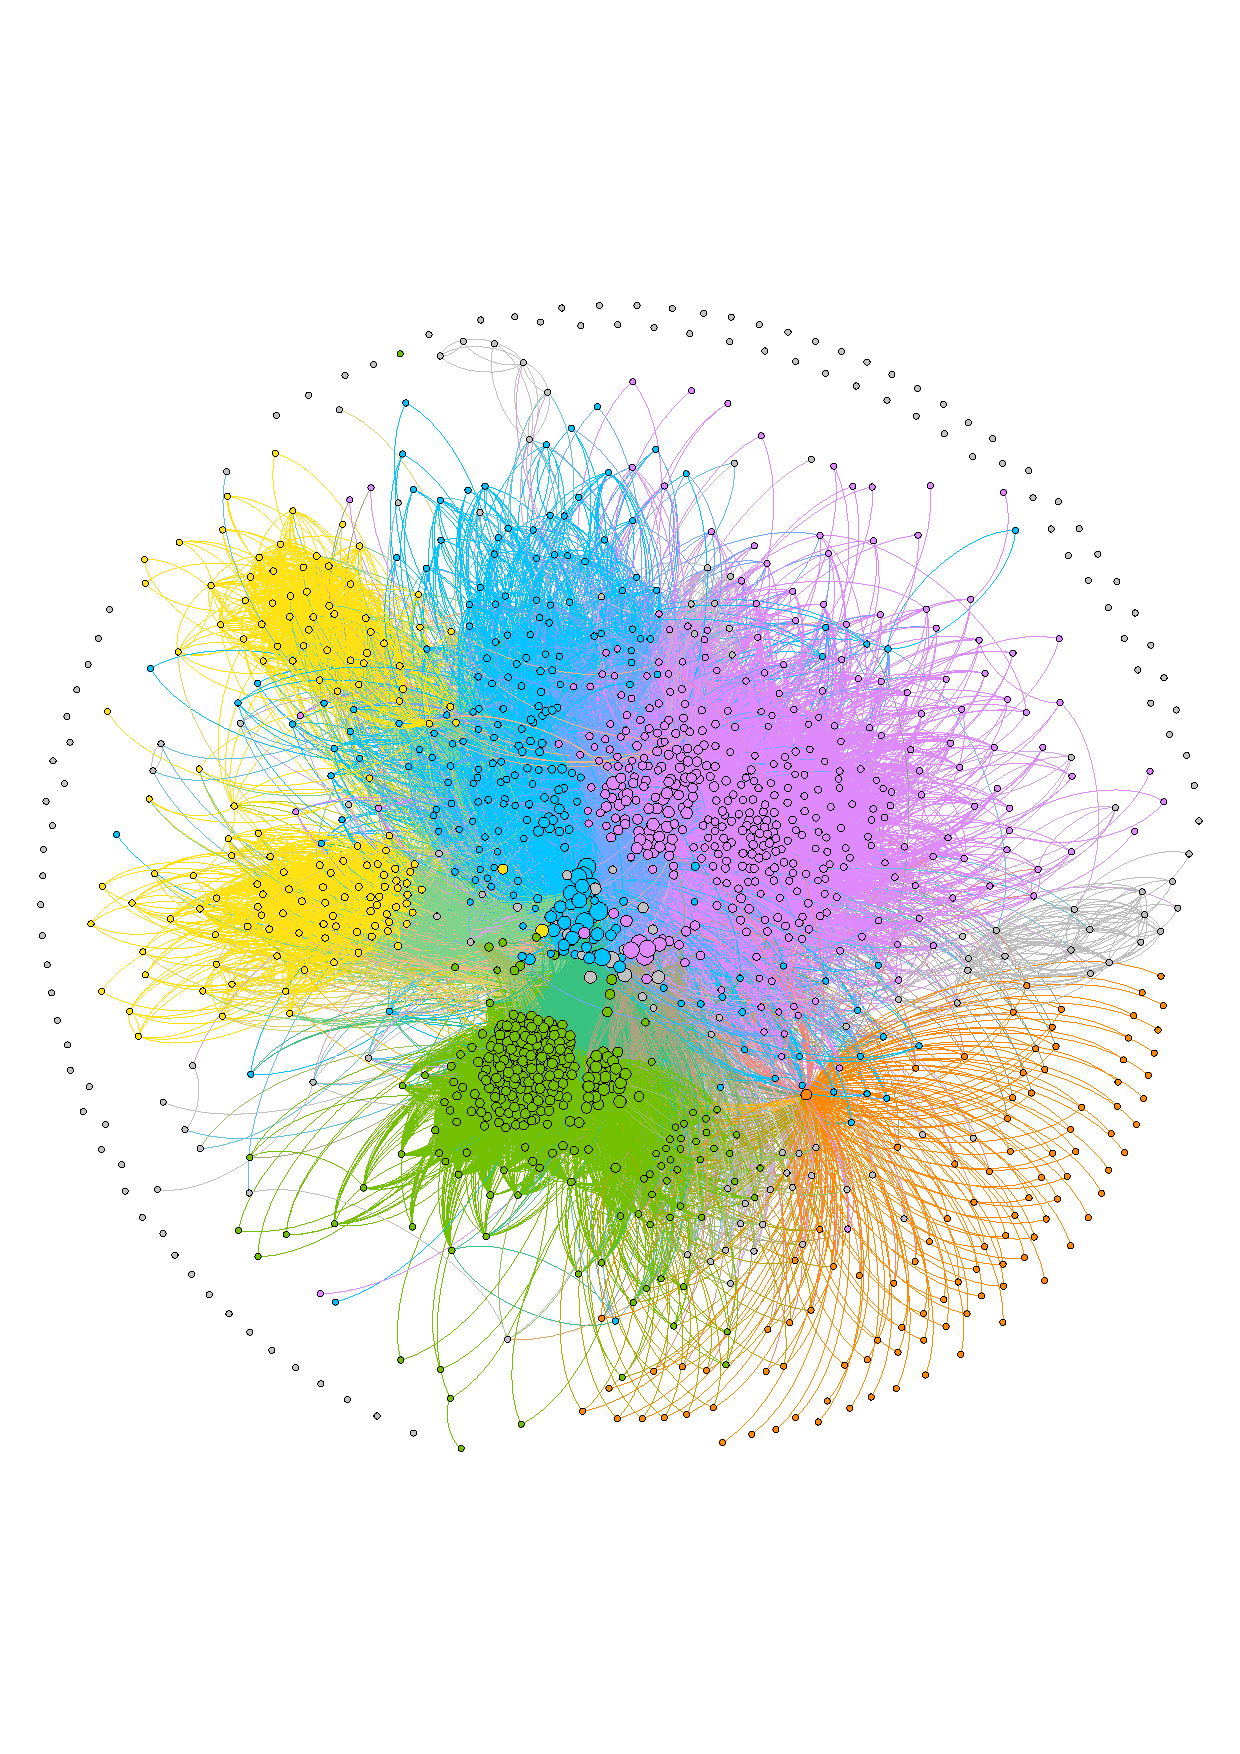
\includegraphics[width=14cm]{community_graph}
	\end{center}
	\caption{Community structure of the 2016 US stock price return network. Five distinct communities are detected represented by different colours of nodes. The direction of edge is  clockwise. The size of nodes and thickness of edges are related to the value of degrees and weights. The grey nodes do not belong to any communities and most of them have zero degree.}
	\label{fig:community_graph}
\end{figure}

\begin{figure} % 各个单独的群落
	\subfloat[Production]{%
		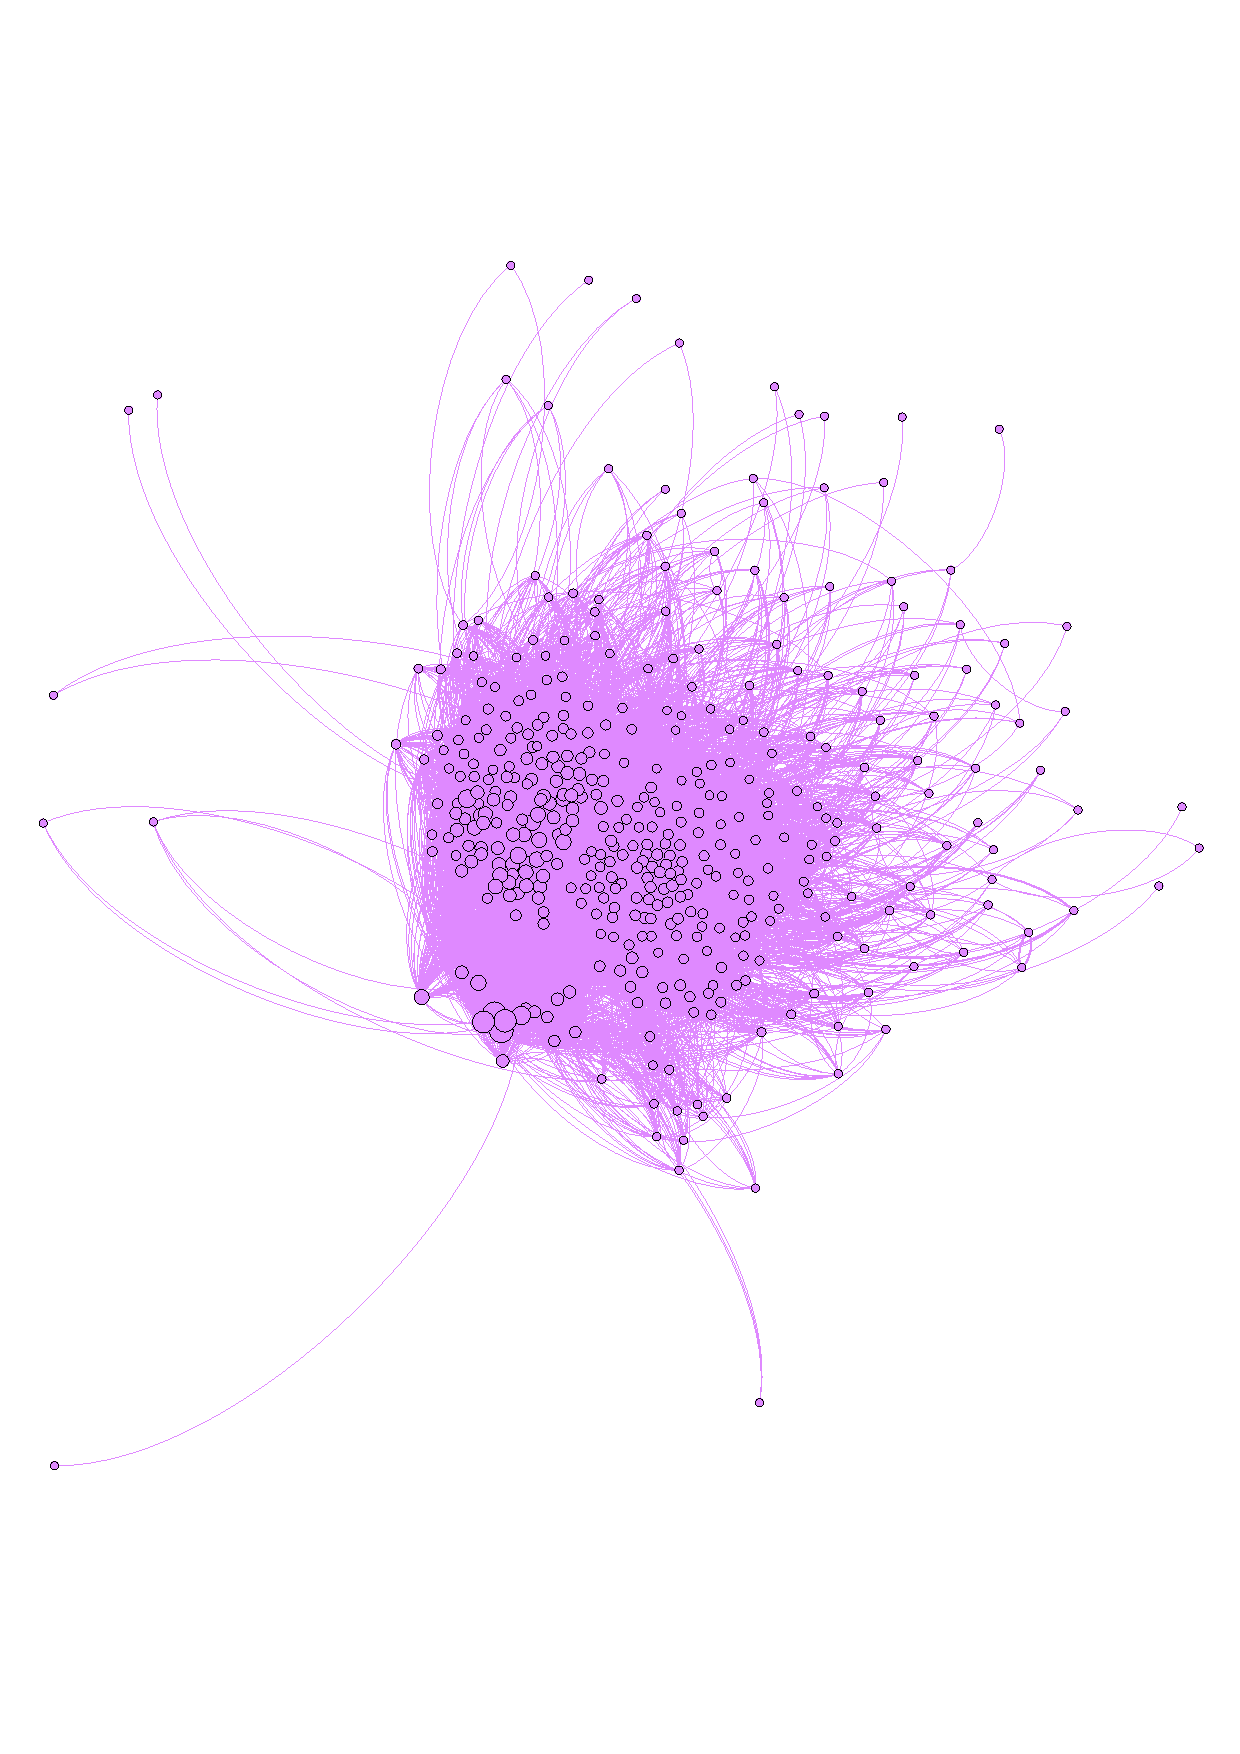
\includegraphics[width=0.46\textwidth]{community_1}%
		\label{fig:community_1}%
	}%
	\hfill%
	\subfloat[Finance]{%
		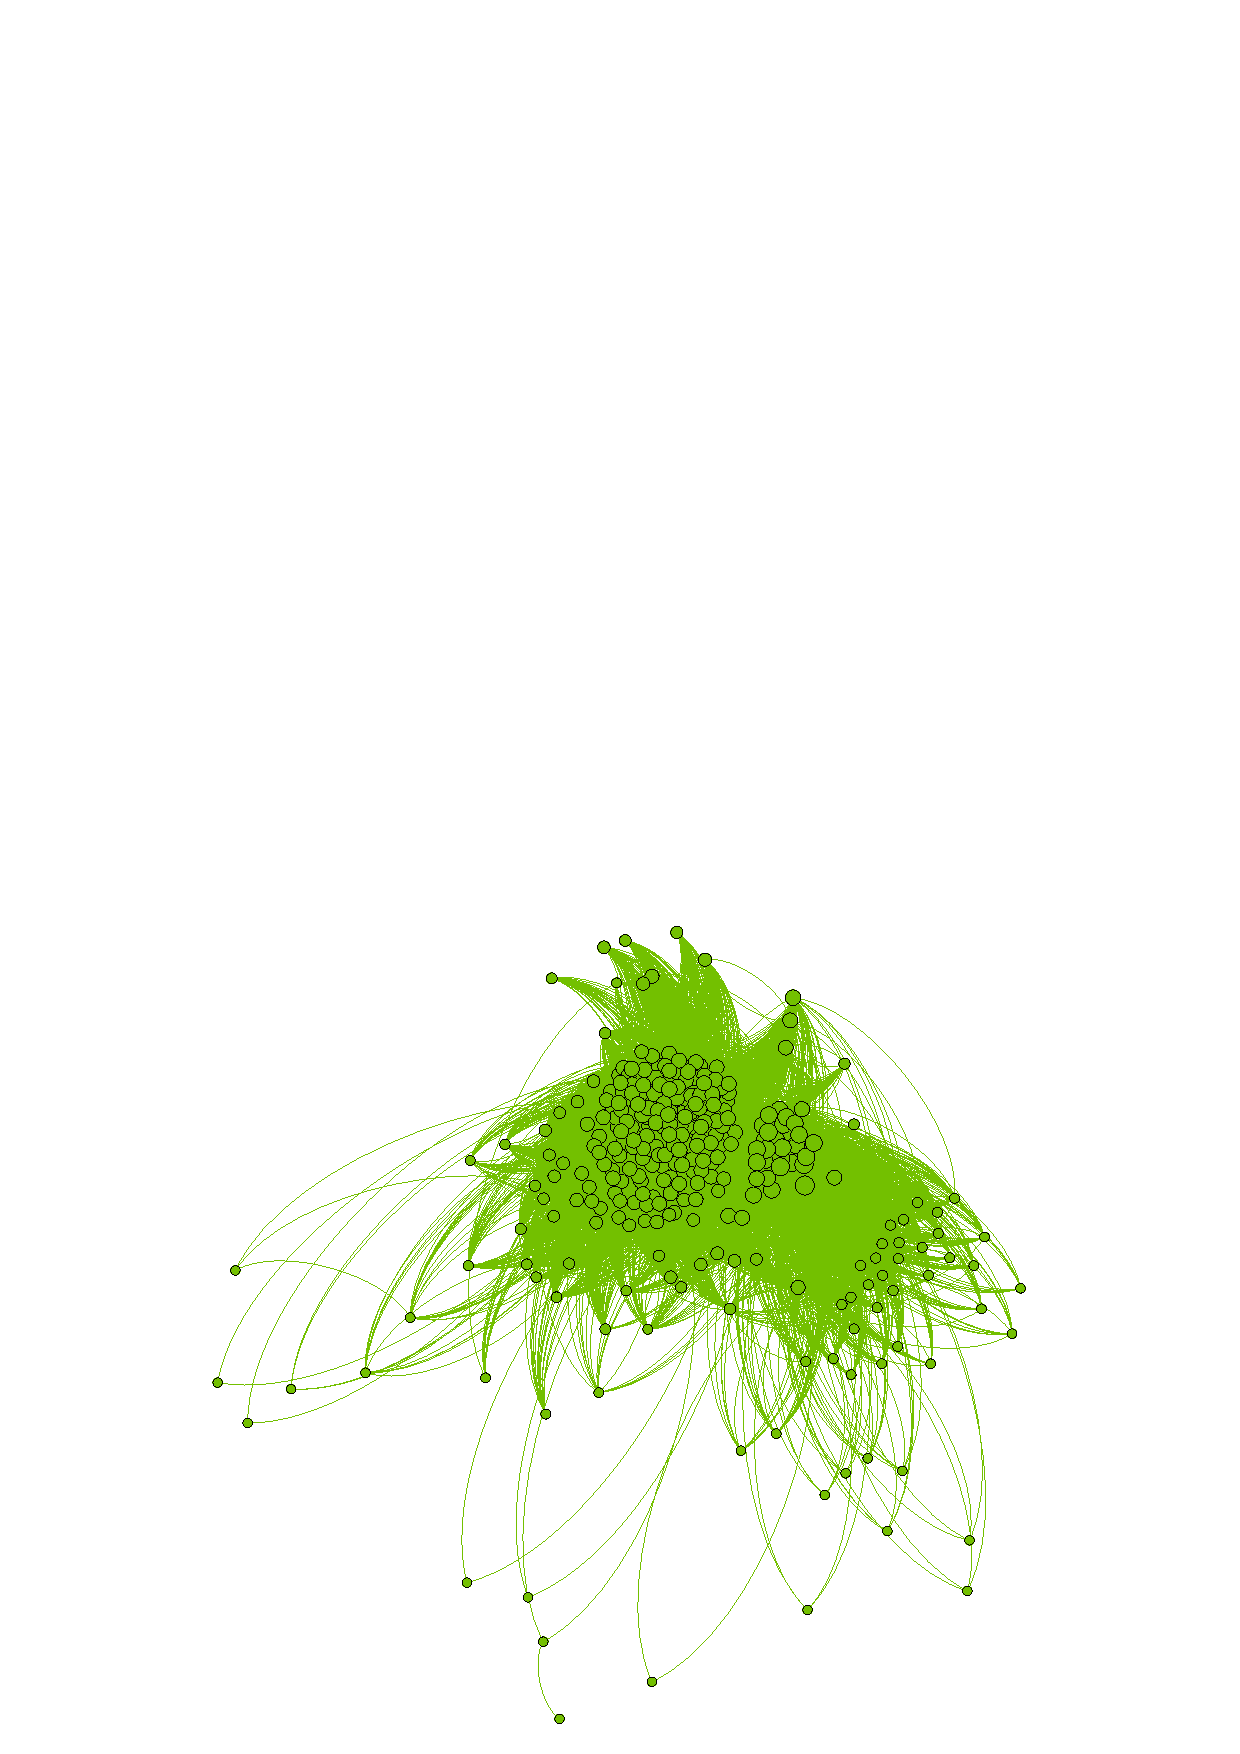
\includegraphics[width=0.46\textwidth]{community_2}%
		\label{fig:community_2}%
	}%
	\hfill%
	\subfloat[Livelihood]{%
		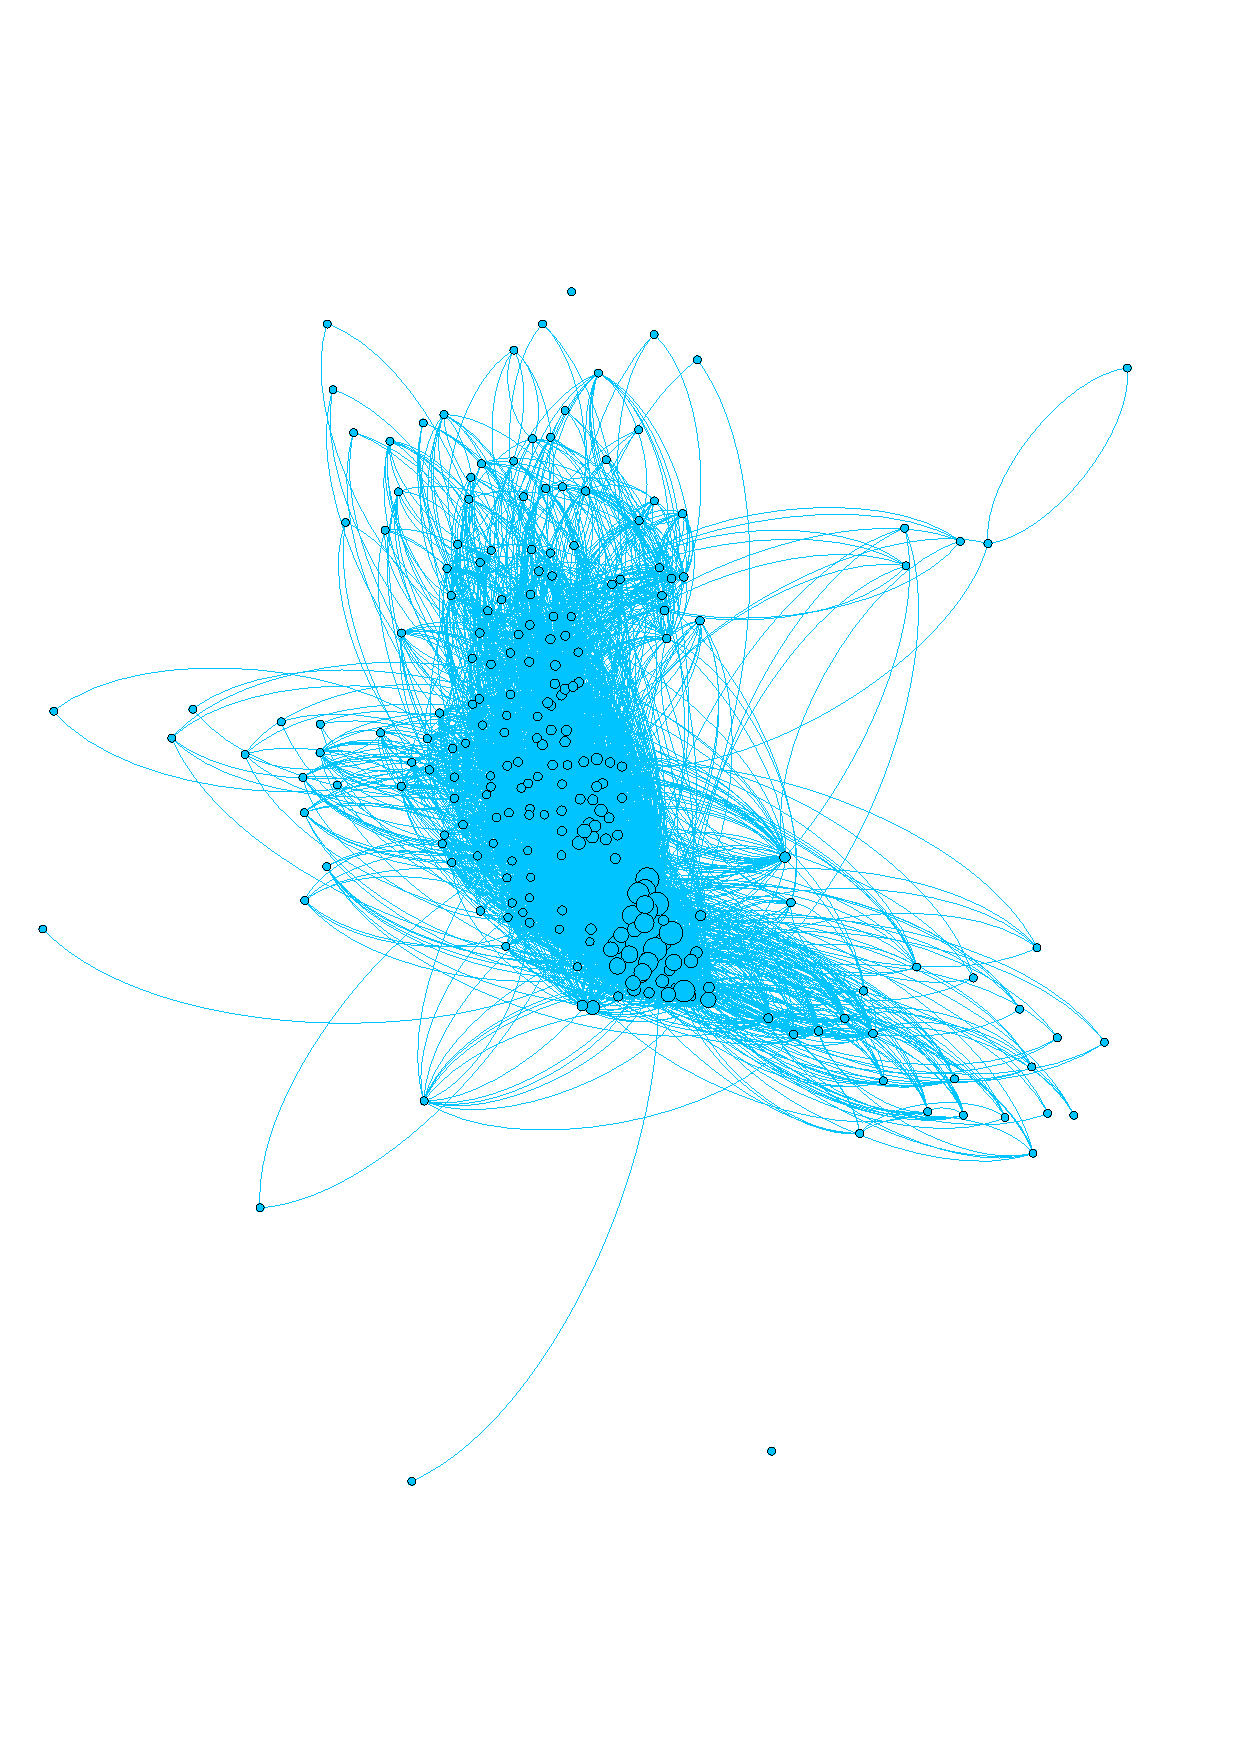
\includegraphics[width=0.46\textwidth]{community_3}%
		\label{fig:community_3}%
	}%
	\hfill%
	\subfloat[Insurance and chemical products]{%
		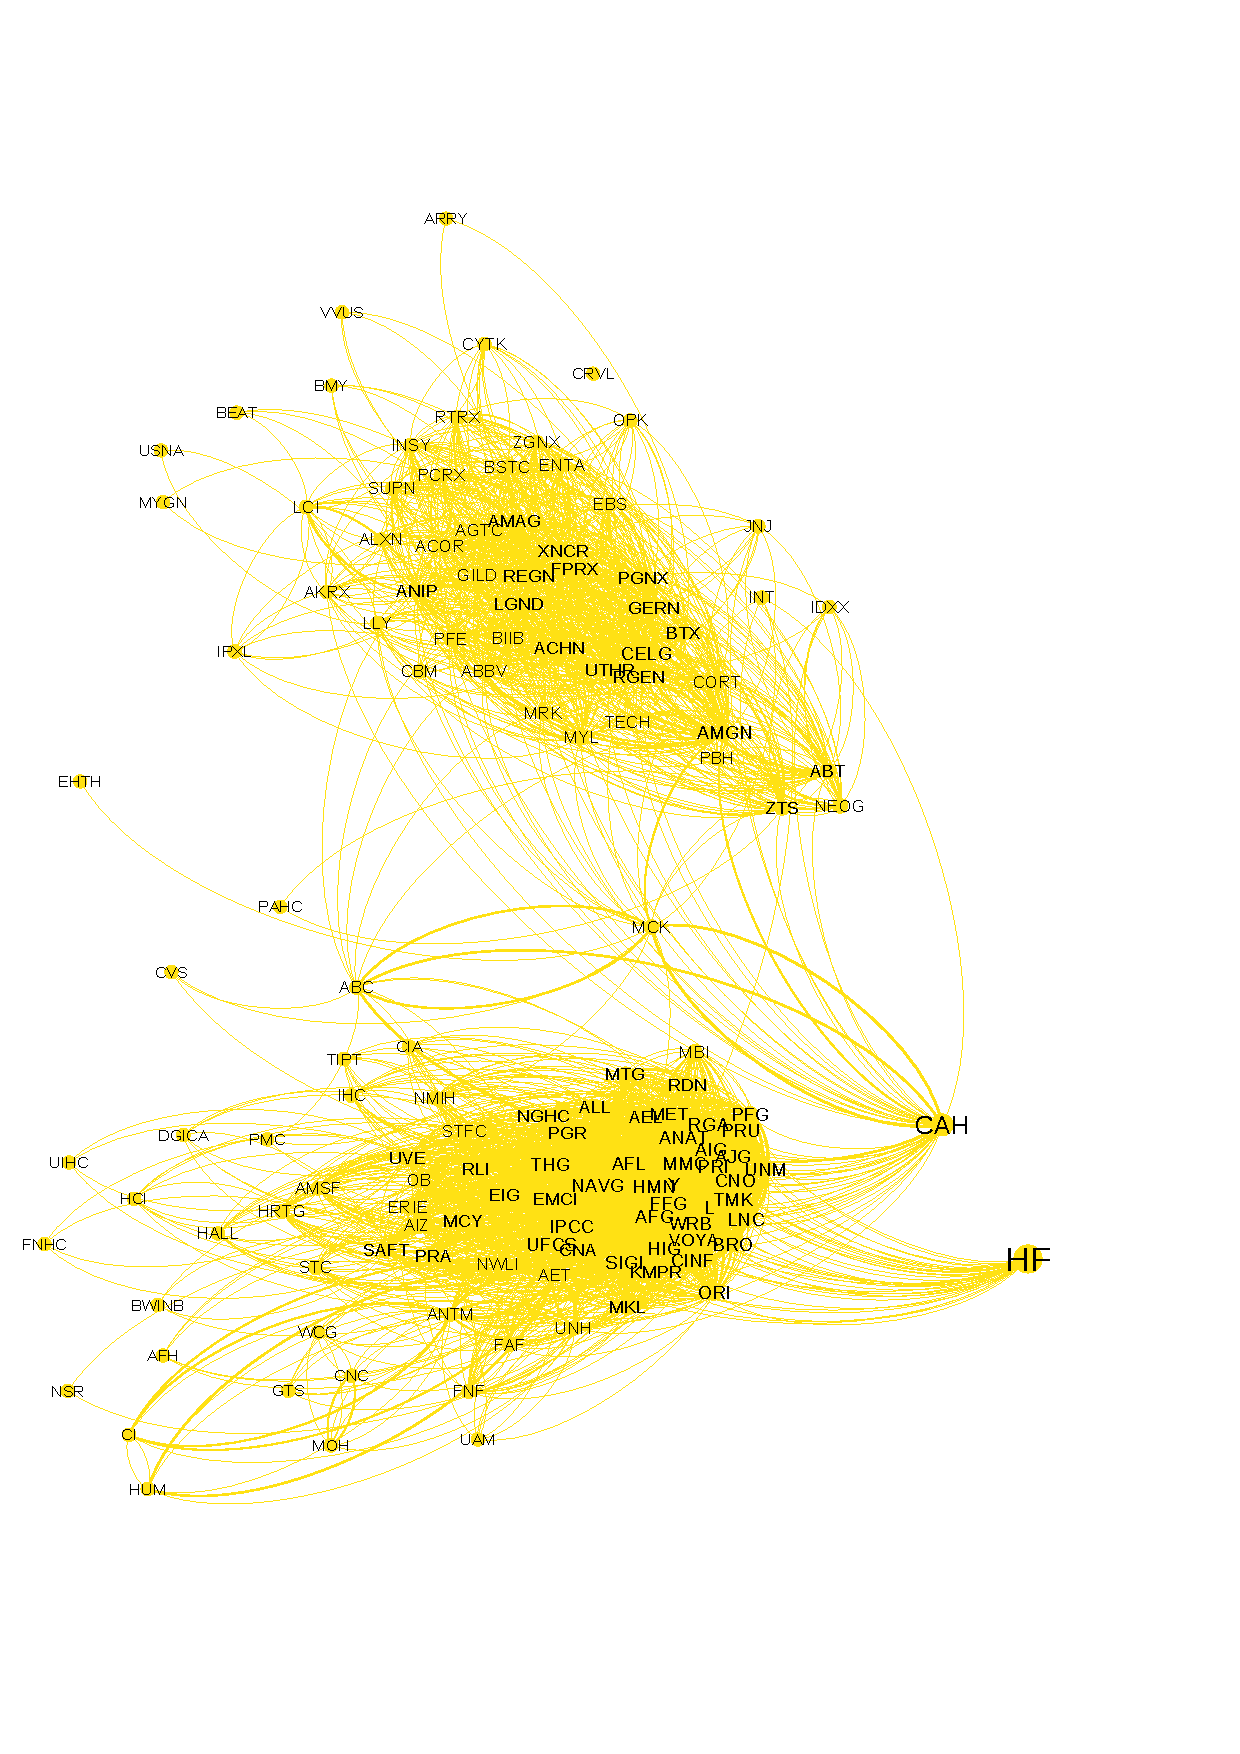
\includegraphics[width=0.46\textwidth]{community_4}%
		\label{fig:community_4}%
	}%
	\hfill%
	\subfloat[Utilities and financial vehicles]{%
		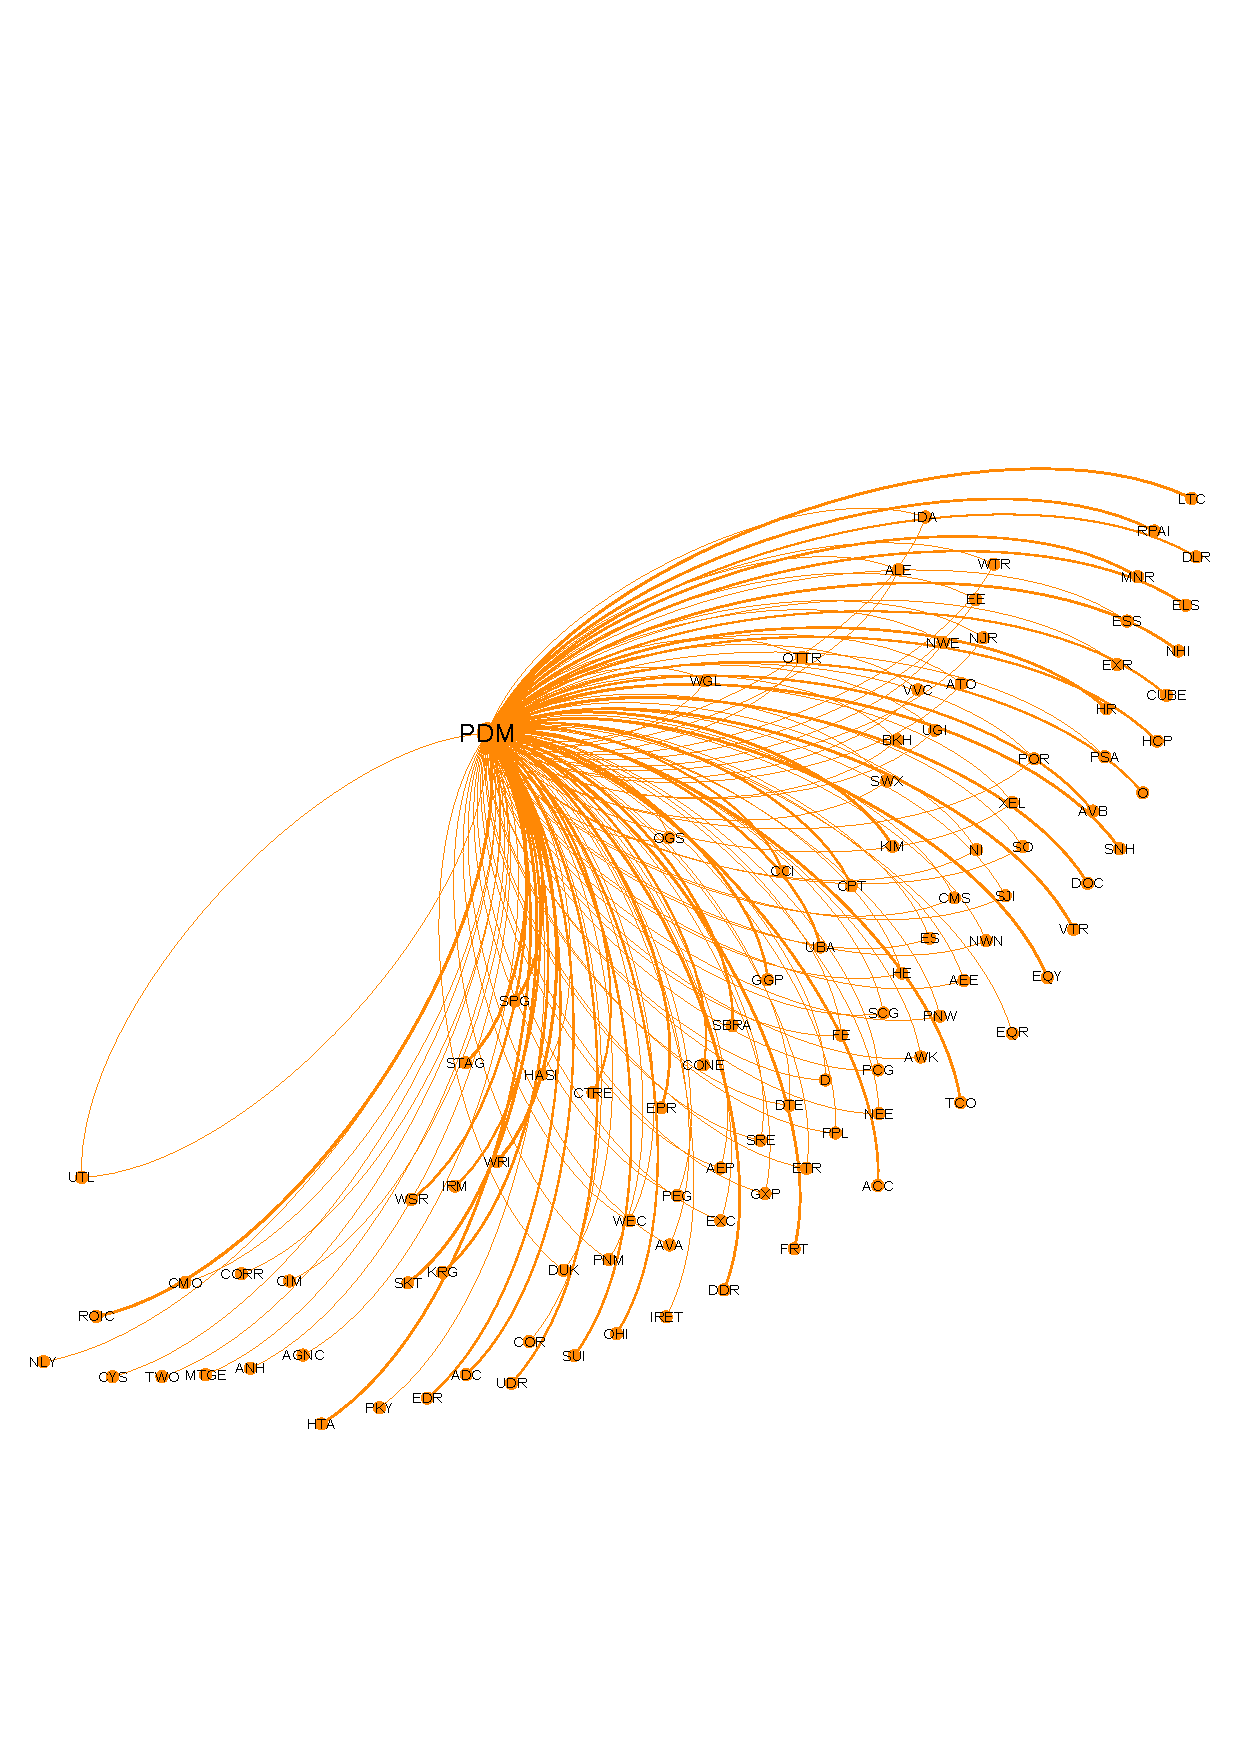
\includegraphics[width=0.46\textwidth]{community_5}%
		\label{fig:community_5}%
	}%
	\caption{Solely community views of the directed stock network. Stock tickers are displayed for the sparsely distributed communities.} \label{fig:distinctcommunities}
\end{figure}

\begin{figure} % 群落的行业柱形图
	\begin{center}
		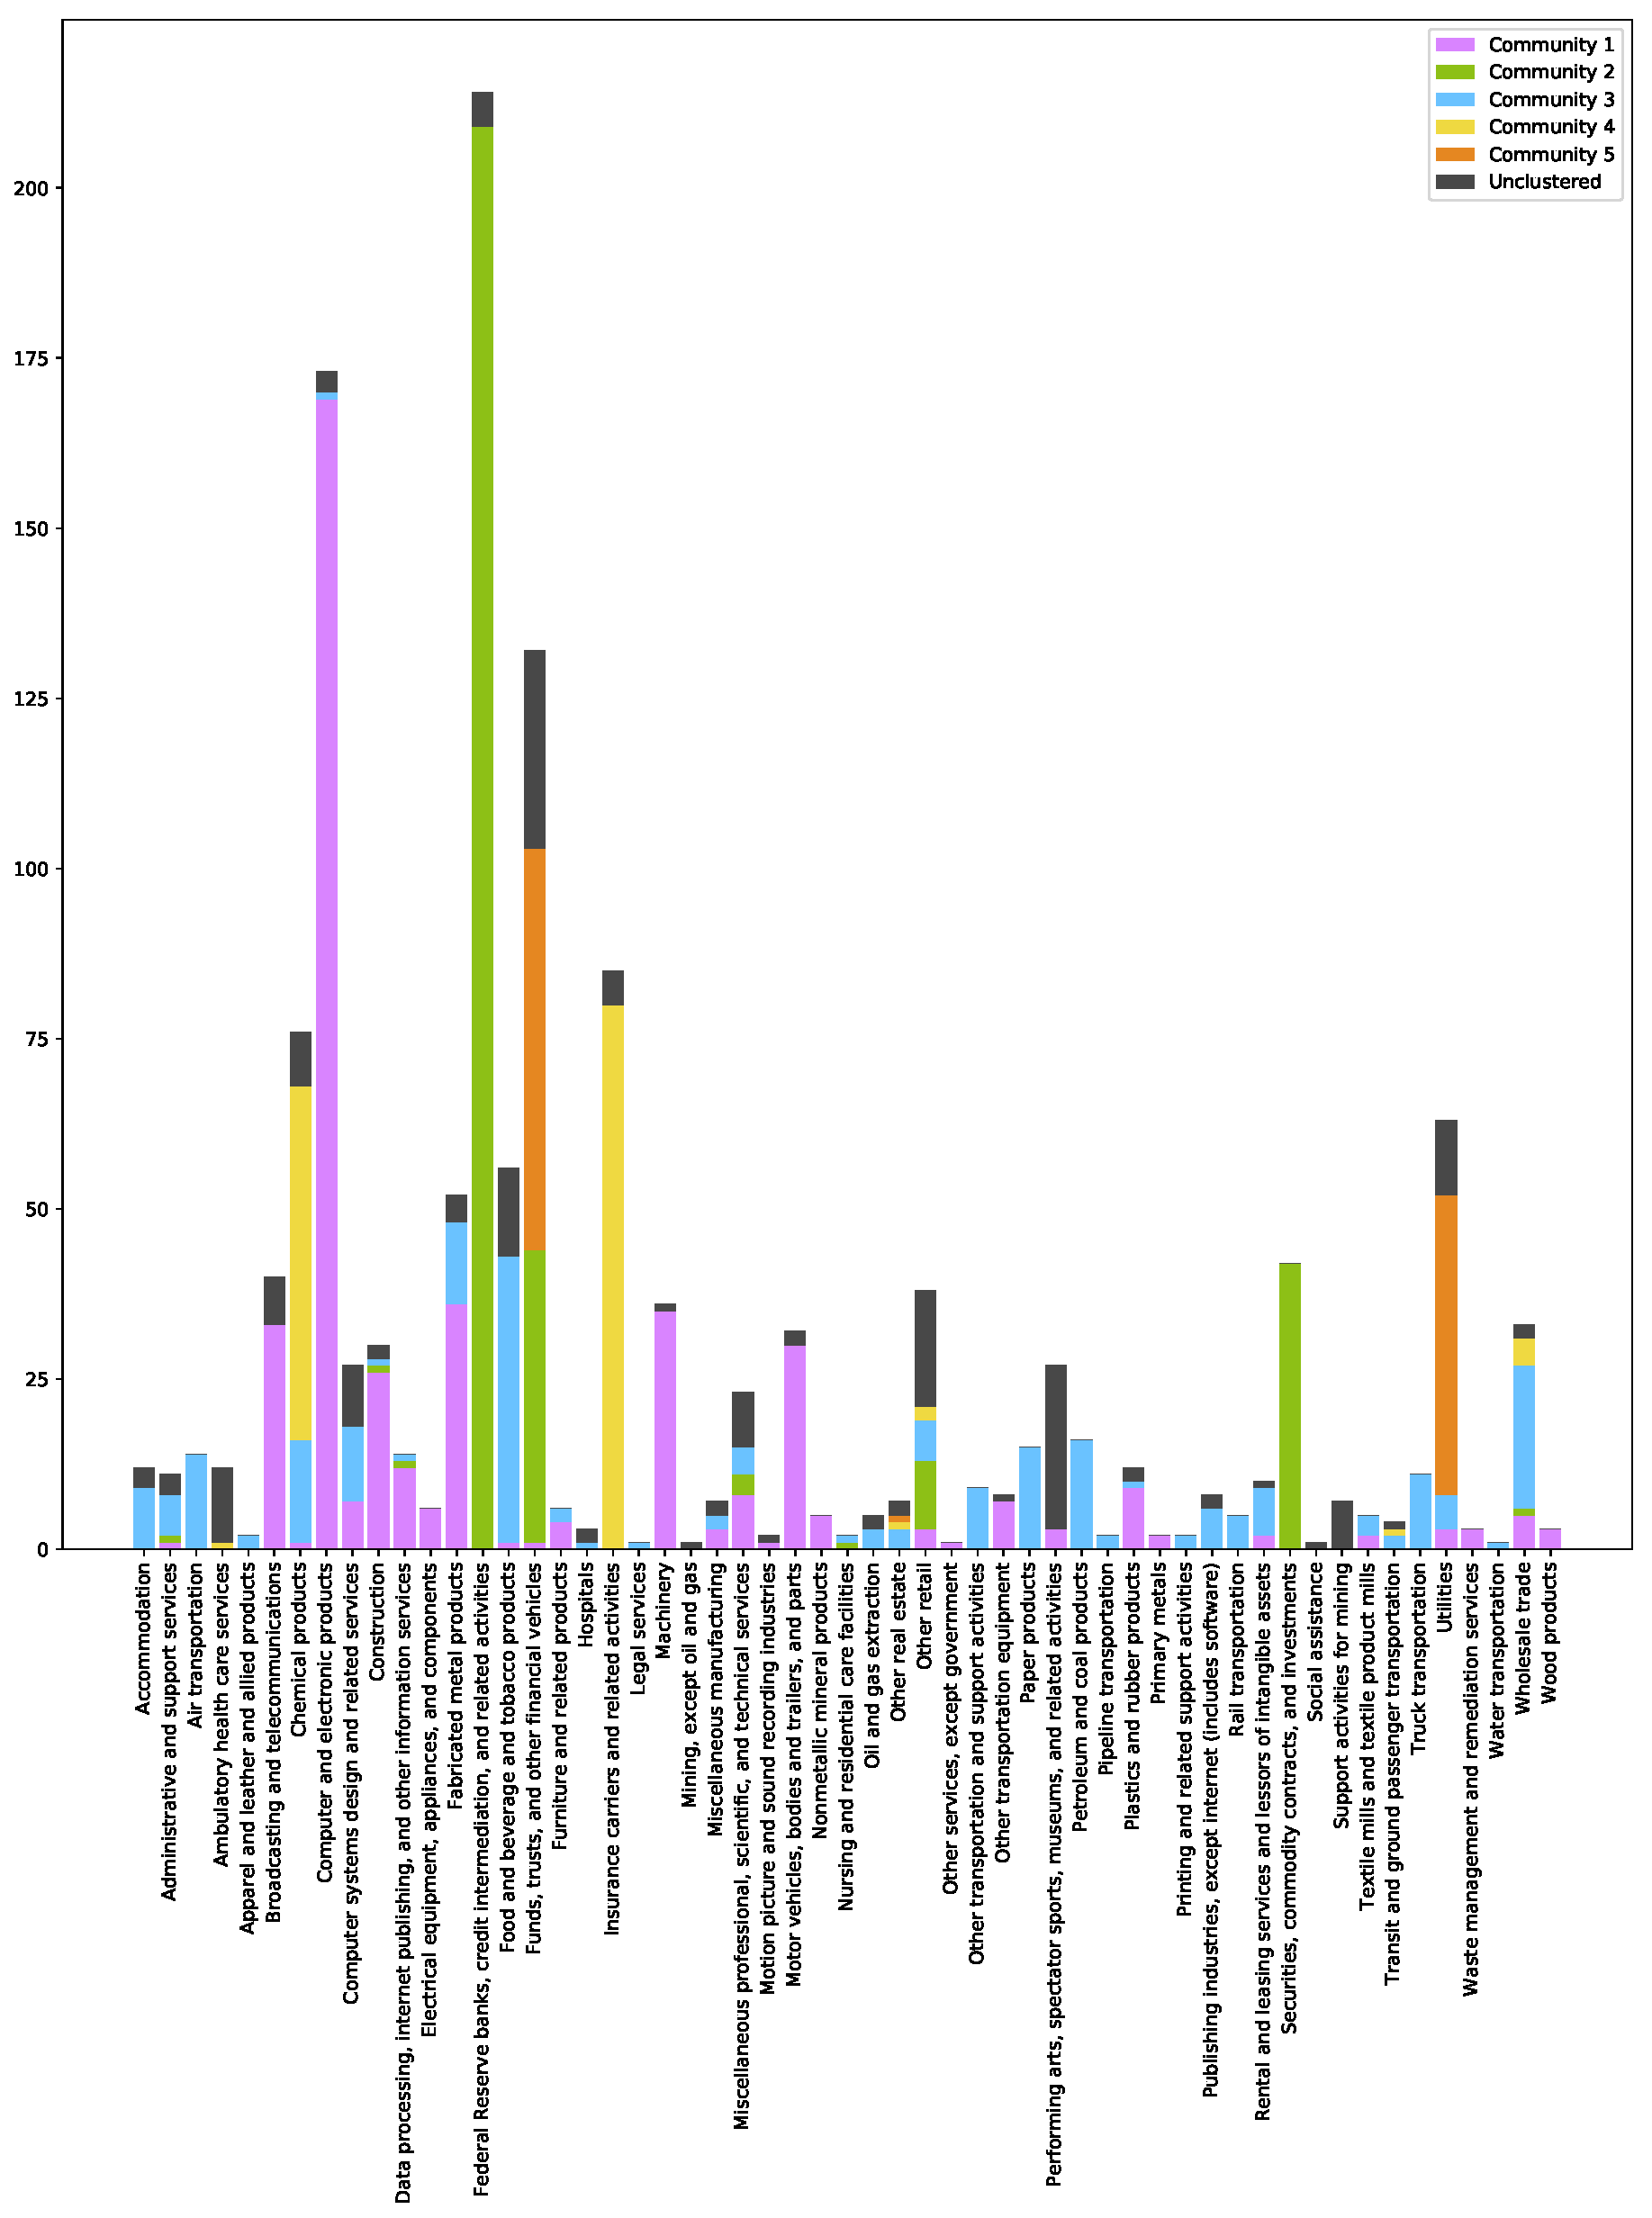
\includegraphics[width=14cm]{community_sector_stacked}
	\end{center}
	\caption{Count of stocks of each communities by industrial sectors. Sectors are arranged alphabetically.}
	\label{fig:community_sector_stacked}
\end{figure}

\begin{table}
	\begin{center}
		\begin{tabular}{|r|c|}\hline\hline
			&Undirected stock network\\\hline
			Degree distribution&Power-law\\
			Average out-degrees&Power-law\\
			Average path length&2.775\\
			Clustering coefficient&0.4675\\
			Global efficiency&0.2563\\
			Local efficiency&0.6276\\
			Assortativity&0.02004\\
			\hline\hline
		\end{tabular}
	\end{center}
	\caption{Main topologies of conventional stock price network}\label{tab:conventional}
\end{table}

\begin{figure}
	\subfloat[Empirical out-degree distribution]{%
		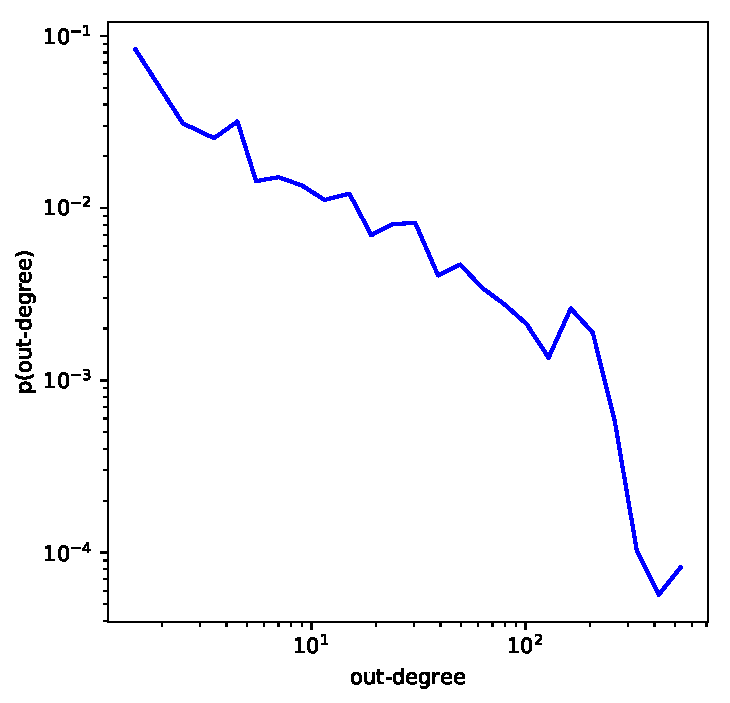
\includegraphics[width=0.46\textwidth]{G_out_degree_distribution_square}%
		\label{fig:G_out_degree_distribution_square}%
	}%
	\hfill%
	\subfloat[CCDF and power-law fit]{%
		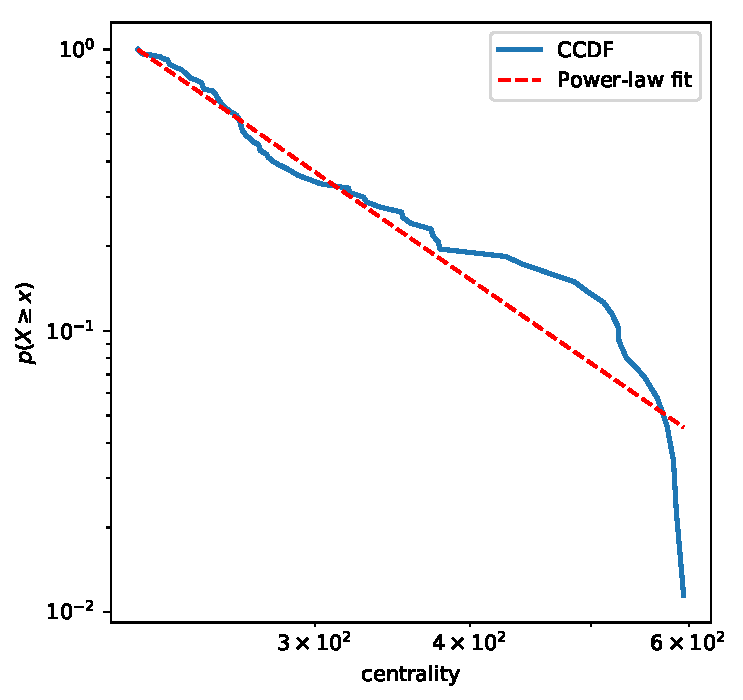
\includegraphics[width=0.465\textwidth]{out_degree_log_fit_square}%
		\label{fig:out_degree_log_fit_square}%
	}%
	\caption{Out-degree distribution of stock network} \label{fig:outdegreedistribution}
\end{figure}

\begin{figure} % P-P SW
	\centering
	\subfloat[Empirical out-degree distribution]{
		\label{subfig:G_sw_out_degree_distribution}
		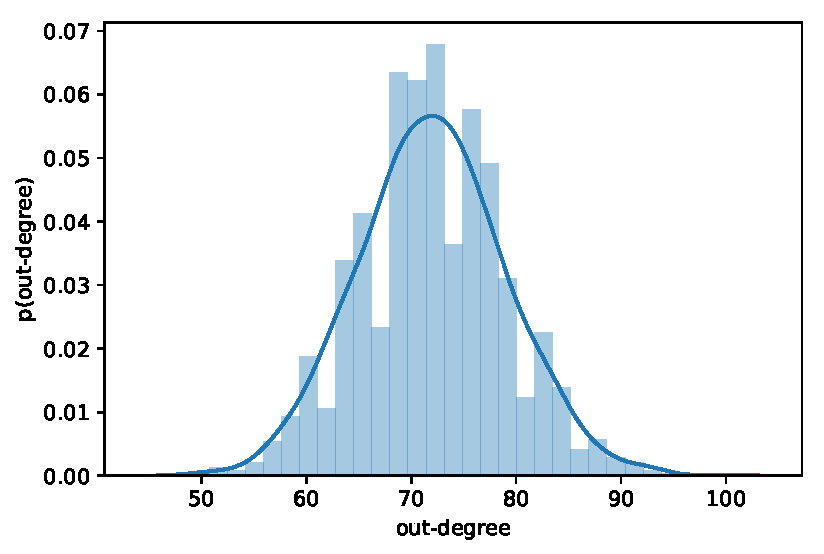
\includegraphics[width=12cm]{G_sw_out_degree_distribution} }
	
	\subfloat[P-P plot]{
		\label{subfig:G_ws_mat_prob_plot}
		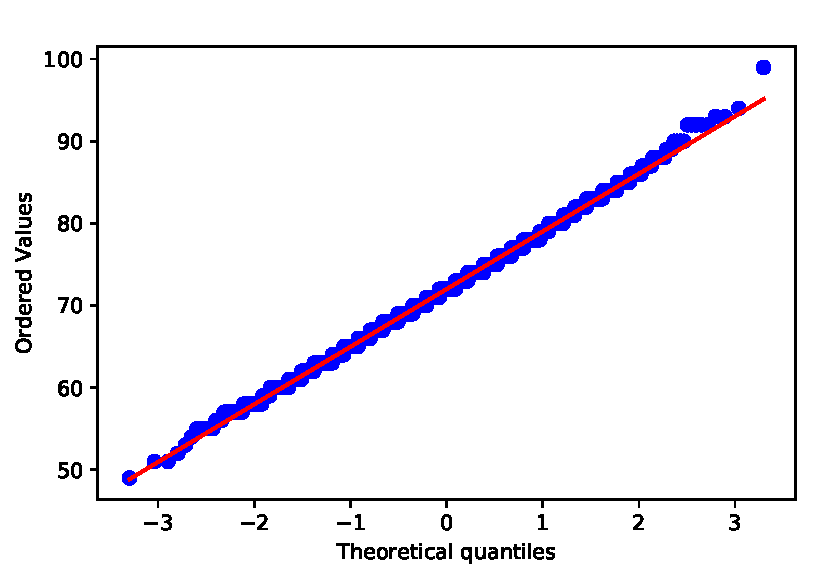
\includegraphics[width=12cm]{G_ws_mat_prob_plot} }
	
	\caption{Out-degree distribution and P-P plot of small-world network}
	\label{fig:distributionsm}
\end{figure}

\begin{figure} % P-P rd
	\centering
	\subfloat[Empirical out-degree distribution]{
		\label{subfig:G_rd_out_degree_distribution}
		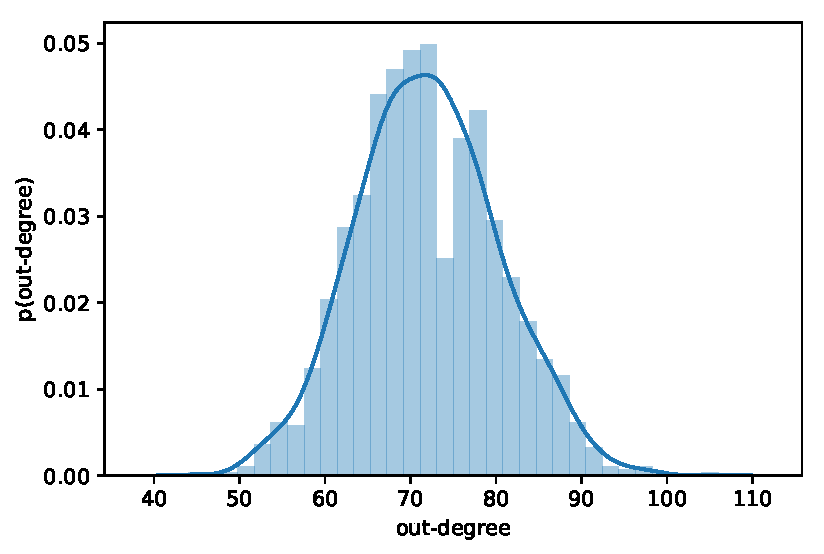
\includegraphics[width=12cm]{G_rd_out_degree_distribution} }
	
	\subfloat[P-P plot]{
		\label{subfig:G_rd_prob_plot}
		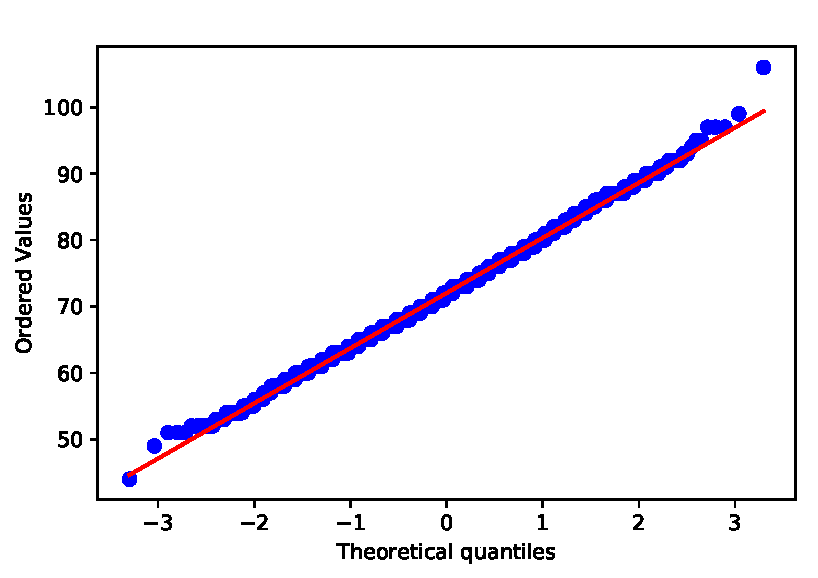
\includegraphics[width=12cm]{G_rd_prob_plot} }
	
	\caption{Out-degree distribution and P-P plot of random network}
	\label{fig:distributionrd}
\end{figure}


\iffalse
\begin{figure}
	\begin{center}
		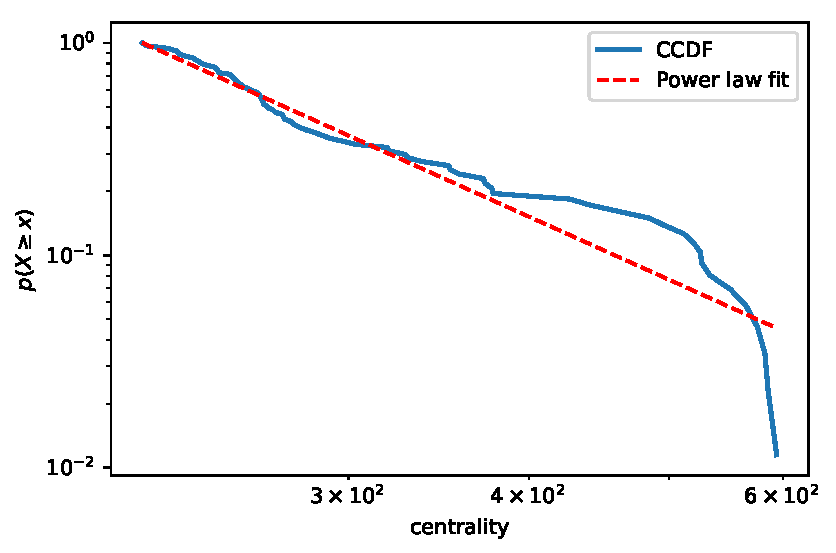
\includegraphics[width=15cm]{out_degree_log_fit}
	\end{center}
	\caption{Amounts of edges per EIO-threshold and correlation-coefficient-threshold}
	\label{fig:out_degree_log_fit}
\end{figure}
\fi

%Clustering coefficient
%行业内非对称边和行业间对称边的数量
%Global/ local efficiency

%Betweenness centrality

%Community detection


\section{Analysis of the directed weighted network}
% Strength distribution
\begin{table}
	\begin{center}
		\begin{tabular}{|r|c|}\hline\hline
			&Undirected stock network\\\hline
			Strength distribution&Power-law\\
			Average centrality&1\\
			Weighted assortativity&0.1244\\
			\hline\hline
		\end{tabular}
	\end{center}
	\caption{Main topologies of directed weighted stock price network}\label{tab:weighted}
\end{table}

\begin{figure} % P-P sw
	\centering
	\subfloat[Bivariate distribution of cumulative sum of daily return]{
		\label{subfig:sum_return_centrality}
		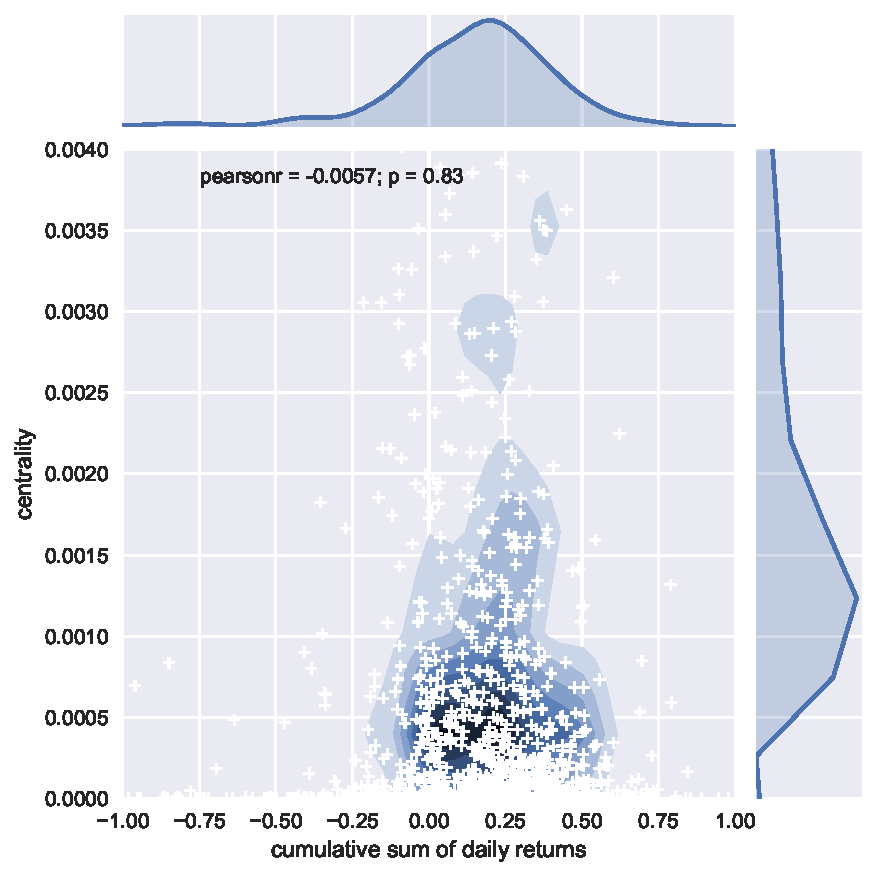
\includegraphics[width=10cm]{sum_return_centrality} }
	
	\subfloat[Bivariate distribution of standard deviation of daily return]{
		\label{subfig:std_return_centrality}
		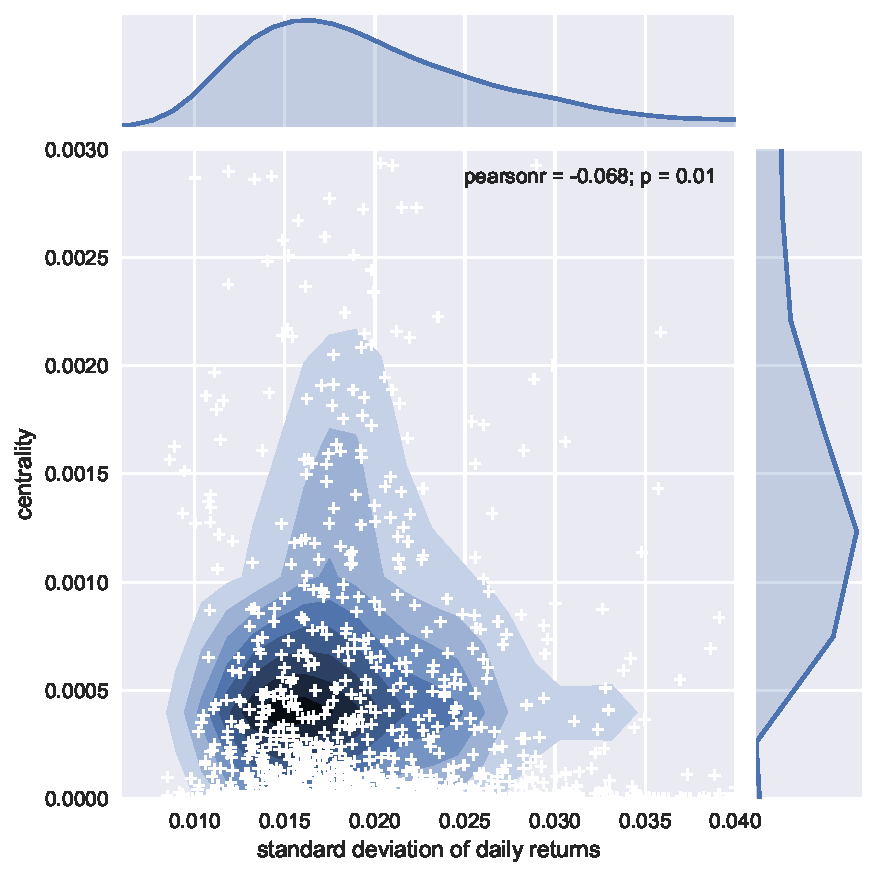
\includegraphics[width=10cm]{std_return_centrality} }
	
	\caption{Bivariate distribution}
	\label{fig:bivariate}
\end{figure}

% Assortativity with weight 0.12444731038165072



% Topological robustness
% Abnormal return regression with topological features as factors
\subsection{Analysis on the relationship between price return and clustering coefficient}


%\section{Community detection}
%\label{sec:community}
%命名各个community
\section{Stability of network}

%Industry

